% bei Standalone in documentclass noch:
% \RequirePackage{luatex85}

\documentclass[captions=tableheading, titlepage= firstiscover, parskip = half , bibliography=totoc]{scrartcl}
%paper = a5 für andere optinen
% titlepage= firstiscover
% bibliography=totoc für bibdateien
% parskip=half  Veränderung um Absätze zu verbessern

\usepackage{scrhack} % nach \documentclass
\usepackage[aux]{rerunfilecheck}
\usepackage{polyglossia}
\usepackage[style=numeric, backend=biber]{biblatex} % mit [style = alphabetic oder numeric] nach polyglossia
\addbibresource{lit.bib}
\setmainlanguage{german}

\usepackage[autostyle]{csquotes}
\usepackage{amsmath} % unverzichtbare Mathe-Befehle
\usepackage{amssymb} % viele Mathe-Symbole
\usepackage{mathtools} % Erweiterungen für amsmath
\usepackage{fontspec} % nach amssymb
% muss ins document: \usefonttheme{professionalfonts} % für Beamer Präsentationen
\usepackage{longtable}

\usepackage[
math-style=ISO,    % \
bold-style=ISO,    % |
sans-style=italic, % | ISO-Standard folgen
nabla=upright,     % |
partial=upright,   % /
]{unicode-math} % "Does exactly what it says on the tin."
\setmathfont{Latin Modern Math}
% \setmathfont{Tex Gyre Pagella Math} % alternativ

\usepackage[
% die folgenden 3 nur einschalten bei documenten
locale=DE,
separate-uncertainty=true, % Immer Fehler mit ±
per-mode=symbol-or-fraction, % m/s im Text, sonst \frac
]{siunitx}

% alternativ:
% per-mode=reciprocal, % m s^{-1}
% output-decimal-marker=., % . statt , für Dezimalzahlen

\usepackage[
version=4,
math-greek=default,
text-greek=default,
]{mhchem}

\usepackage[section, below]{placeins}
\usepackage{caption} % Captions schöner machen
\usepackage{graphicx}
\usepackage{grffile}
\usepackage{subcaption}

% \usepackage{showframe} Wenn man die Ramen sehen will

\usepackage{float}
\floatplacement{figure}{htbp}
\floatplacement{table}{htbp}

\usepackage{mhchem} %chemische Symbole Beispiel: \ce{^{227}_{90}Th+}


\usepackage{booktabs}

 \usepackage{microtype}
 \usepackage{xfrac}

 \usepackage{expl3}
 \usepackage{xparse}

 % \ExplSyntaxOn
 % \NewDocumentComman \I {}  %Befehl\I definieren, keine Argumente
 % {
 %    \symup{i}              %Ergebnis von \I
 % }
 % \ExplSyntaxOff

 \usepackage{pdflscape}
 \usepackage{mleftright}

 % Mit dem mathtools-Befehl \DeclarePairedDelimiter können Befehle erzeugen werden,
 % die Symbole um Ausdrücke setzen.
 % \DeclarePairedDelimiter{\abs}{\lvert}{\rvert}
 % \DeclarePairedDelimiter{\norm}{\lVert}{\rVert}
 % in Mathe:
 %\abs{x} \abs*{\frac{1}{x}}
 %\norm{\symbf{y}}

 % Für Physik IV und Quantenmechanik
 \DeclarePairedDelimiter{\bra}{\langle}{\rvert}
 \DeclarePairedDelimiter{\ket}{\lvert}{\rangle}
 % <name> <#arguments> <left> <right> <body>
 \DeclarePairedDelimiterX{\braket}[2]{\langle}{\rangle}{
 #1 \delimsize| #2
 }

\setlength{\delimitershortfall}{-1sp}

 \usepackage{tikz}
 \usepackage{tikz-feynman}

 \usepackage{csvsimple}
 % Tabellen mit \csvautobooktabular{"file"}
 % muss in table umgebung gesetzt werden


% \multicolumn{#Spalten}{Ausrichtung}{Inhalt}

\usepackage{hyperref}
\usepackage{bookmark}
\usepackage[shortcuts]{extdash} %nach hyperref, bookmark

\newcommand{\ua}[1]{_\symup{#1}}
\newcommand{\su}[1]{\symup{#1}}


\title{Versuch 354}
\subtitle{Gedämpfte und erzwungene Schwingungen}
\author{Sebastian Pape\\
        sepa@gmx.de \and
        Jonah Nitschke\\
        lejonah@web.de}
\date{Durchführung: 01.02.2017\\
      Abgabe: 08.02.2017}

\begin{document}

\maketitle
\newpage

\section{Theorie}

In dem folgenden Versuch wird ein elektronischer Kreis, im Kern bestehend aus einem
Widerstand, einer Spule und einem Kondensator. Über diese Schaltung kann eine
gedämpfte Schwingung betrachtet werden, sowie durch Anschluss eines Generators
aus eine erzwungene Schwingung. Im Laufe des Versuches sollen der Dämpfungswiderstand,
die Frequenzabhängigkeit der Kondensatorspannung sowie die Phase zwischen
Erreger- und Kondensatorspannung betrachtet werden.

\subsection{Der gedämpfte Schwingkreis}

Der in diesem Experiment betrachtete gedämpfte Schwingkreis ist in Im Grunde nur
eine Erweiterung des RC-Kreise mit einer Spule. Somit kommen in der Schaltung
zwei Energiespeicher vor, zwischen denen die Energie hin und her pendelt. Durch
den eingebauten Widerstand geht bei der Schwingung Energie in Form von Wärme verloren
und somit wird das ganze System gedämpft. Betrachtet man solch eine Schaltung, kann
mithilfe der Kirchhoffschen Gesetze eine Differentialgleichung für den Strom
aufgestellt werden:

\begin{equation}
  \frac{\su{d}^2I}{\su{d}t^2} + \frac{R}{L}\frac{\su{d}I}{\su{d}t} + \frac{1}{LC} I = 0 .
\end{equation}

Durch Lösen der Differentialgleichung ergibt sich mit einem geeigneten Ansatz für
die Frequenz ein Term, der von der Stärke der Dämpfung abhängig ist:

\begin{equation}
  \tilde{\omega}_{1,2} = j \frac{R}{2L} \pm \sqrt{ \frac{1}{LC} - \frac{R^2}{4L^2}} .
\end{equation}

Je nachdem wie sich der unter der Wurzel stehende Term verhält, können für die
gedämpfte Schwingung verschiedene Fälle betrachtet werden, von denen zwei im folgenden
Erläutert werden.

\textbf{1.Fall :} $\frac{1}{LC} > \frac{R^2}{4L^2}$

In diesem Fall ist der Term mit der Wurzel rein reel und  es entsteht eine
harmonische Schwingung, deren Amplitude mit zunehmender
Zeit gegen Null geht. Die Einhüllende wird dabei durch eine Exponentialfunktion
beschrieben, wie auch in Abbildung \ref{fig:Schwingfall} anhand der rot gestrichelten
Linie zu sehen ist.
Mithilfe der Schwingungsdauer lässt sich dann errechnen, nach welcher
Zeit die Amplitude auf den $e$-ten Teil ihrer Ursprungsamplitude abgesenkt ist:

\begin{equation}
  T\ua{ex} := \frac{2L}{R} \su{s} .
\end{equation}

\begin{figure}
  \centering
  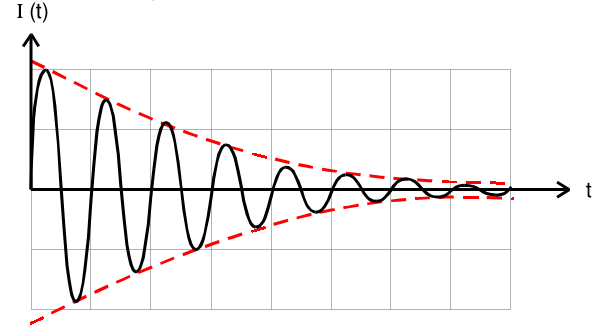
\includegraphics{Schwingfall.png}
  \caption{Zeitlicher Verlauf einer gedämpften Schwingung}
  \label{fig:Schwingfall}
\end{figure}

\textbf{2.Fall :} $\frac{1}{LC} < \frac{R^2}{4L^2}$

Bei diesem Fall handelt es sich um eine aperiodische Dämpfung, bei der die Lösung
keinen oszillatorischen Teil besitzt. In diesem Versuch wird dabei nur der als
aperiodischer Grenzfall bezeichneter Spezialfall betrachtet, bei dem
$\frac{1}{LC} = \frac{R^2}{4L^2}$ gilt und der Strom ohne Überschwinger am schnellsten
gegen Null geht (siehe schwarz gestrichelte Linie Abbildung \ref{fig:Kriechfall}).

\begin{figure}
  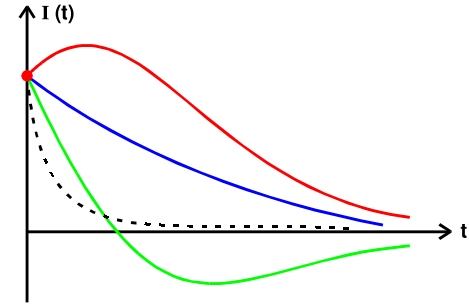
\includegraphics{Kriechfall.png}
  \caption{Möglicher Zeitverlauf des Stromes in einem Schwingkreis mit aperiodischer Dämpfung}
  \label{fig:Kriechfall}
\end{figure}

\newpage

\subsection{Die erzwungene Schwingung}

Wird bei dem vorher betrachteten Schaltkreis noch ein Generator mit eingebaut,
handelt es sich um eine erzwungene Schwingung, für die sich mithilfe der
Kirchhoffschen Gesetze für die Kondensatorspannung $U\ua{C}$
folgende Differentialgleichung ergibt:

\begin{equation}
  LC\frac{\su{d}^2U\ua{C}}{\su{d}t^2} + RC\frac{\su{d}U\ua{C}}{\su{d}t} + U\ua{C} = U\ua{0} \exp^{j\omega t} .
\end{equation}

Aus dieser Differentialgleichung können nun mit einem geeigneten Ansatz eine Funktion
für die Kondensatorspannung $U\ua{c}$ sowie eine Gleichung für die Phasenverschiebung
$\varphi$ zwischen Erreger- und Kondensatorspannung bestimmt werden:

\begin{align}
  \varphi(\omega) &= \arctan \left( \frac{-\omega RC}{1 - LC\omega^2} \right) \\
  U\ua{C}(\omega) &= \frac{U\ua{0}}{ \sqrt{ \left(1 - LC\omega^2 \right)^2 + \omega^2R^2C^2}} .
\end{align}

Die Kondensatorspannung kann bei der sogenannten Resonanzfrequenz $\omega\ua{res}$
auch einen Wert größer als $U\ua{0}$ annehmen:

\begin{equation}
  \omega\ua{res} = \sqrt{\frac{1}{LC} - \frac{R^2}{2L^2}} .
\end{equation}

Wird bei der Schaltung eine schwache Dämpfung betrachtet, für die
$\frac{R^2}{2L^2} \, << \, \frac{1}{LC}$ gilt, nähert sich $\omega\ua{res}$
der Kreisfrequenz $\omega\ua{0}$ der ungedämpften Schwingung an. In diesem
Fall übertrifft $U\ua{C}$ die Erregerspannung $U\ua{0}$ um den Faktor
$\frac{1}{\omega\ua{0}RC}$, welcher auch als Güte $q$ des Schwingkreises bezeichnet wird.

Ein weiterer Faktor für die Güte eines Schwingkreises ist die Breite der Resonanzkurve,
welche durch die beiden Frequenzen $\omega\ua{+}$ und $\omega\ua{-}$ charakterisiert
wird. Bei den beiden Frequenzen handelt es sich um die Werte, bei denen die
Kondensatorspannung auf den Bruchteil $\frac{1}{\sqrt{2}}$ ihres Maximalwertes
absinkt. Für Güte und Breite folgt dabei folgende Beziehung:

\begin{equation}
  q = \frac{\omega\ua{0}}{\omega\ua{+} - \omega\ua{-}} .
\end{equation}

\newpage

\section{Durchführung}

Im ersten Teil des Experimentes wird die Zeitabhängigkeit der Amplitude untersucht,
um daraus den effektiven Dämpfungswiderstand zu bestimmen. Dafür wird die Schaltung
aus Abbildung \ref{fig:MessungA} verwendet. Dabei wird auf dem Oszilloskop die abklingende Schwingung
beobachtet. Mithilfe des Reglers wird die Zeitachseneinstellung so angepasst, bis
auf dem Bildschirm ein Intervall zu sehen ist, auf dem die Amplitude etwa um
den Faktor 3 bis 8 abgenommen hat. Anschließend werden mit der Cursor sowohl
Amplituden der Maxima sowie auch der zeitliche Abstand gemessen und ein Thermodruck
angefertigt.

\FloatBarrier
\begin{figure}
  \centering
  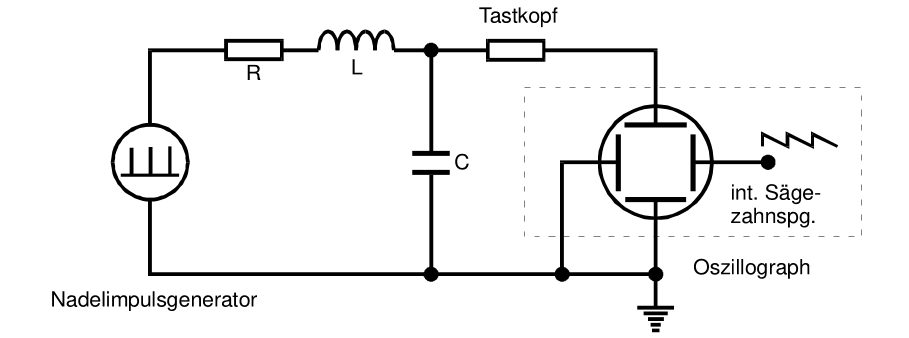
\includegraphics{MessungA.png}
  \caption{Schaltung zur Messung der Zeitabhängigkeit der Kondensatorspannungsamplitude}
  \label{fig:MessungA}
\end{figure}
\FloatBarrier

Im zweiten Fall wird die Schaltung aus Abbildung \ref{fig:MessungB} verwendet, bei der nun der
veränderbare Widerstand in den Stromkreis angeschlossen wird. Der Widerstand wird
zu erst auf maximalen Wert eingestellt, so das auf dem Bildschirm eine aperiodische
Dämpfung beobachtbar ist. Dann wird der Widerstand so lange runter geregelt, bis
auf dem Oszilloskop ein Überschwinger zu sehen ist. Der Dämpfungswiderstand ist
dabei genau in dem Moment eingestell, wo gerade noch kein Überschwinger zu erkennen
ist.

\FloatBarrier
\begin{figure}
  \centering
  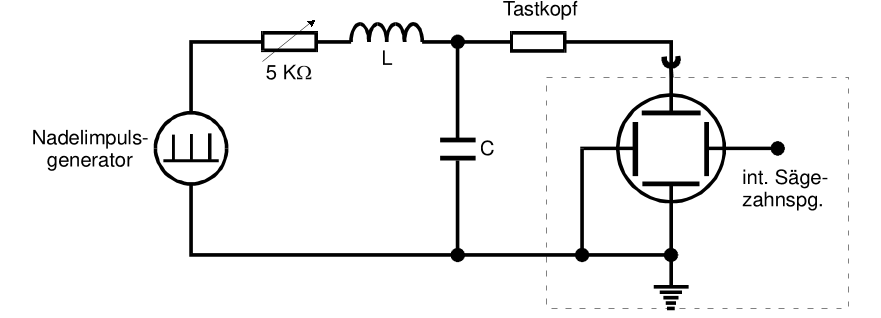
\includegraphics{MessungB.png}
  \caption{Schaltung zur Bestimmung des Dämpfungswiderstandes bei dem aperiodischen Grenzfall}
  \label{fig:MessungB}
\end{figure}
\FloatBarrier

Für die letzten beiden Teile der Messung wird der Schaltplan aus Abbildung \ref{fig:MessungC} verwendet.
Auf dem Oszilloskop werden dabei sowohl die Erreger- als auch die Kondensatorspannung
sichtbar gemacht. Zuerst werden bei jeder Frequenzveränderung die Amplituden beider
Spannungen notiert. Dann werden mithilfe des Cursors der zeitliche Abstand der beiden
Nulldurchgänge beider Spannungsverläufe sowie die Wellenlänge der Kondensatorspannung
gemessen, um daraus hinterher die Phasenverschiebung zu berechnen.

\FloatBarrier
\begin{figure}
  \centering
  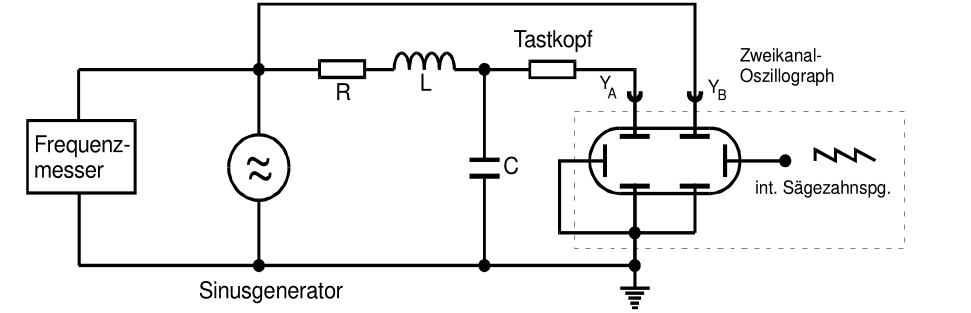
\includegraphics{MessungC.png}
  \caption{Schaltung zur Messung der Frequenzabhängigkeit sowie der Phasenverschiebung}
  \label{fig:MessungC}
\end{figure}
\FloatBarrier

\end{document}
